\documentclass[10pt,letterpaper]{article}

\usepackage[margin=0.75in]{geometry}
\usepackage{tikz}
\usepackage{graphicx}
\usepackage{amsmath}
\graphicspath{{img/}}
\begin{document}

  \title{Stats 314, Data Analysis \#2}
  \author{Cody Malick\\
  \texttt{malickc@oregonstate.edu}}
  \date{\today}
  \maketitle

\section*{Part I}
\subsection*{a}
The dataset with the smallest standard deviation is 'iii.' The reason being
all the numbers are the same. The standard deviation is a quantity calculated
to indicated the extent of deviation for the entire dataset. If they're all the
same number, then the standard deviation of the dataset is 0.

\subsection*{b}
The set with the largest standard deviation will be the one with the most
values far away from the mean. In this case, 'i' would have the largest standard
deviation because of the numbers '7' and '11.' Seven and eleven are the only
differences between the two datasets. Because these two values 'deviate' from
mean more than the values in dataset 'ii,' then 'i' has a larger standard
deviation.

\section*{Part II}
Scheme B would be better because even numbers of both barley populations get
an even amount of water from the river. The main issue with scheme B is that
two of type 1 barley could get all the land by the river, encouraging growth.\\

Scheme B would create two groups of even barley groups. One with both types
getting water, and one with both types not getting water. Scheme B, as stated
above, would be susceptible to an uneven distribution of samples with and without
water.

\section*{Part III}
\subsection*{a}
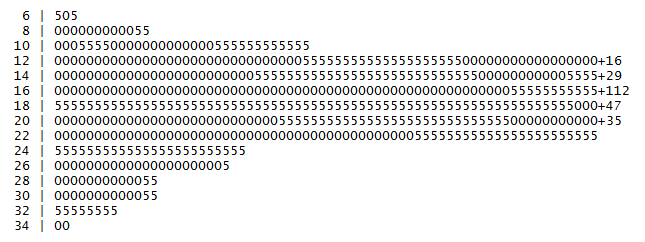
\includegraphics[scale=.5]{stem}\\
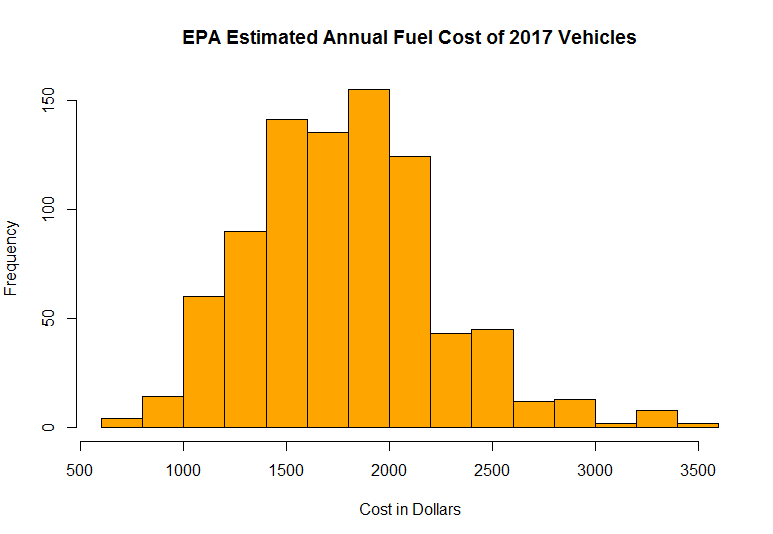
\includegraphics[scale=.5]{hist}\\
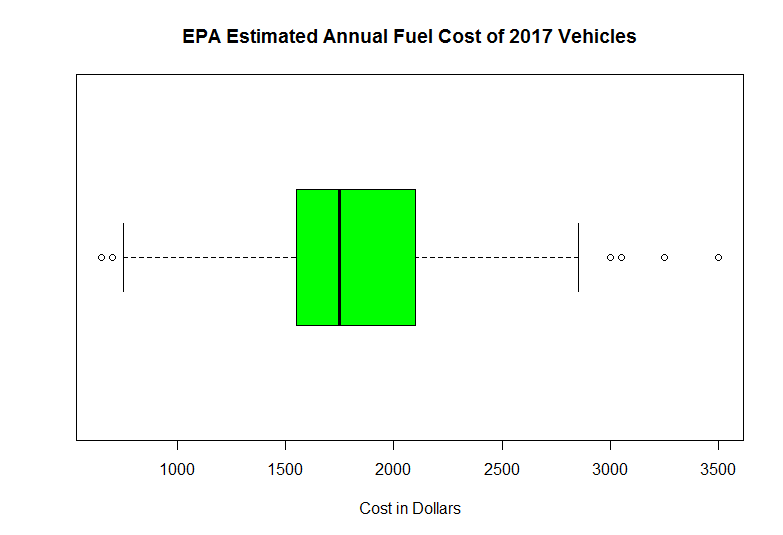
\includegraphics[scale=.5]{box}\\\\
I feel that the stem and leaf plot is not appropriate for this typ e of data 
set. The histogram does an excellent job showing where the data is most 
concentrated, as well as being visually intuitive. The only issue being it's
not readily clear what the exact median is. The box plot, on the other hand,
while not being entirely intuitive visually, immediately gives some clear
measurements about what parts of the data we care about, and what parts are
irrelevant. I would say in this case that the histogram is the best choice.
\subsection*{b}
No, because there are too many values to make the stem and leaf plot useful.
\subsection*{c}
It represents the area between the first and third quartiles.
\subsection*{d}
\begin{tabular}{ l | c | c | c | c | c | c | r }
	Mean & Standard Deviation & Minimum & 1st Quartile & median & 3rd quartile & maximum & IQR\\ \hline
	1815 & 459.428 & 650 & 1550 & 1750 & 2100 & 3500  & 550 
\end{tabular}
\subsection*{e}
The data has a single mode, with a positively skewed shape. There were a few
outliers as we approach the maximum around 3000 to 3500. The center is the
median at 1750.
\subsection*{f}
In this case, either the mean (1815) or the median (1750) could be argued to be
great metrics. The reason for this is that the distribution of the data is
fairly grouped around the median/mean. They both land in the second quartile,
and are near the top of the mode. 
\section*{Part IV}
\subsection*{a}
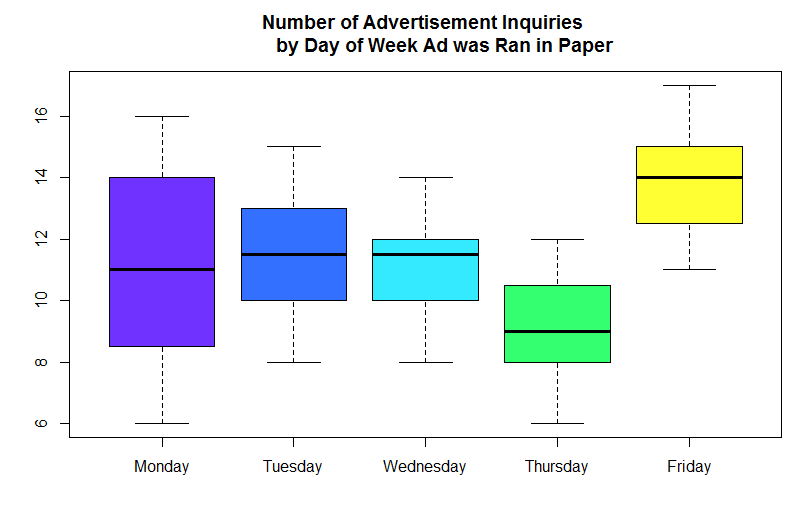
\includegraphics[scale=.5]{colorbox}
\subsection*{b}
\begin{tabular}{ l | c | c | c | r }
	Day & Inquires.Min & Inquiries.1st Quartile & Inquiries.Median & Standard Deviation\\ \hline
	Monday & 6.00 & 8.75 & 11.00 & 3.315 \\ \hline
	Tuesday & 8.00 & 10.00 & 11.50 & 2.067 \\ \hline
	Wednesday & 8.00 & 10.00 & 11.50 & 1.696 \\ \hline
	Thursday & 6.00 & 8.00 & 9.00 & 1.758 \\ \hline
	Friday & 11.00 & 12.75 & 14.00 & 1.781 \\ 
\end{tabular}

\subsection*{c}
At first glance the visually intuitive answer is that Friday is the best day to
run an add in the paper. The reason for this being that the IRQ is very high
compared to any of the other days. The majority of the data lies in a high
range. Looking at the median for that day, it also places much, much higher than
the other days. Looking at the data in our table, it also indicates that friday
is a better day because of the median and the minimum.
\subsection*{d}
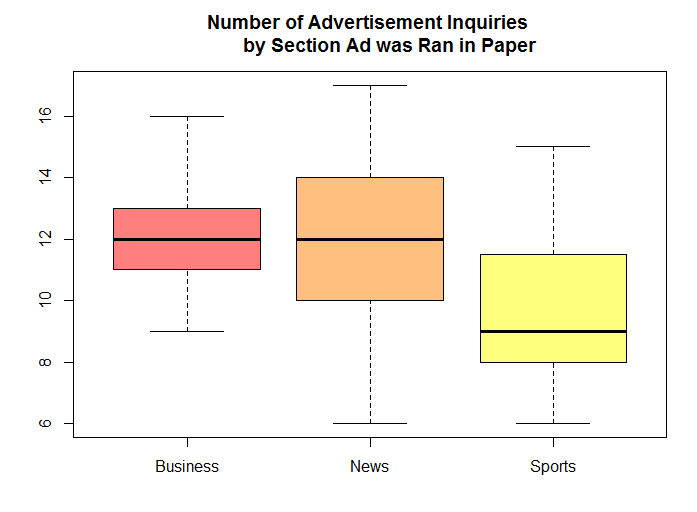
\includegraphics[scale=.5]{sectionBox}
\subsection*{e}
\begin{tabular}{ l | c | c | c | r }
	Section & Inquires.Min & Inquiries.1st Quartile & Inquiries.Median & Standard Deviation\\ \hline
	Business & 9.00 & 11.00 & 12.00 & 1.744 \\ \hline
	News & 6.00 & 10.50 & 12.00 & 3.059 \\ \hline
	Sports & 10.00 & 11.25 & 15.00 & 2.575 \\ 
\end{tabular}

\subsection*{f}
At first glance, Business looks like a fairly solid section to run adds in.
The reason for this being that the distance between the first and third
quartiles is fairly small, meaning that most of the ads run that day lie in a
fairly concentrated range. The standard deviation for Business is fairly low.
Looking at News, however, shows that there are days where News will run more
inquiries than business, but also the posibility of less inquiries. Sports, on
the other hand, runs less inquiries in general.
\subsection*{g}
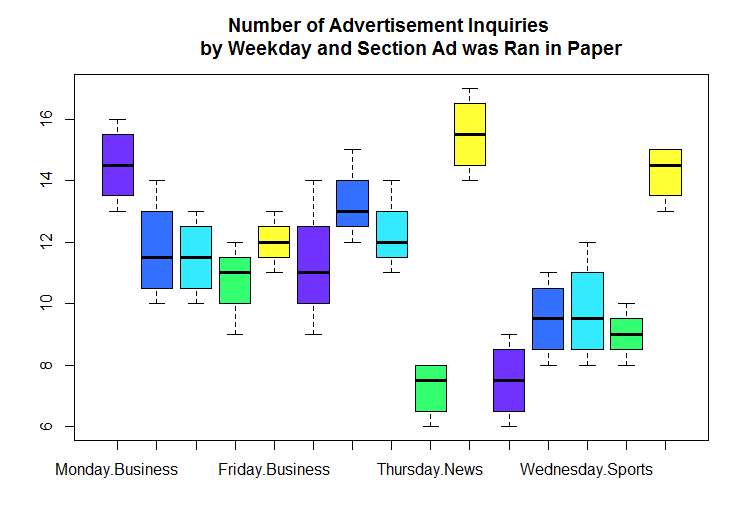
\includegraphics[scale=.5]{multiBox}
\subsection*{h}
\begin{tabular}{ l | c | r }
	Day & Section & Inquires\\ \hline
	Monday & Business & 14.50 \\ \hline
	Tuesday & Business & 11.75 \\ \hline
	Wednesday & Business & 11.50 \\ \hline
	Thursday & Business & 10.75 \\ \hline
	Friday & Business & 12.00 \\ \hline
	Monday & News & 11.25 \\ \hline
	Tuesday & News & 13.25 \\ \hline
	Wednesday & News & 12.25 \\ \hline
	Thursday & News & 7.25 \\ \hline
	Friday & News & 15.50 \\ \hline
	Monday & Sports & 7.50 \\ \hline
	Tuesday & Sports & 9.50 \\ \hline
	Wednesday & Sports & 9.75 \\ \hline
	Thursday & Sports & 9.00 \\ \hline
	Friday & Sports & 14.25 
\end{tabular}

\subsection*{i}
Overall, immediately visible, Friday is one of the best days two out of three
times. Friday, followed by Monday, would be the best two days to place ads
overall. The other days vary throughout the week, but Monday and Friday end up
having the highest average medians. 
\end{document}
